\section{End-to-End Benchmarks}
\label{s:benchmarks}

We start by evaluating the total cost attributable to all mitigations for transient execution attacks.
This value is different for each individual CPU, so we compare both across generations of processors and between vendors.

Later sections will go into more detail on how individual attacks work and the characteristics of their respective mitigations, but for now we wish only to gain a high level understanding of which mitigations are relevant from a performance perspective.

The primary impact of transient execution attacks is to leak information across protection boundaries.
Accordingly mitigations to prevent such leakage often involve extra operations when the CPU transitions from one protection domain to another.
Alternatively, some mitigations must be enabled continuously while untrusted code is being executed.
Based on this, we focus on two particularly relevant protection boundaries: the user-kernel interface for the operating system, and the sandboxing that web browsers' JavaScript engines provide between execution contexts for different sites.
The boundary between a hypervisor and its guest operating system is also notable, but we did not find significant performance differences between running virtualization workloads with and without mitigations enabled.

In addition, we consider the case of a compute-intensive workload running within a single operating system process.
This involves no protection boundary crossings, and thus measures only the impact of mitigations the operating system keeps enabled all the time.

\subsection{Methodology}
In the following benchmarks we evaluate across eight different CPU microarchitectures from two vendors.
Considering different microarchictures enables us to observe design improvements between successive releases.
\autoref{fig:cpus} lists out detailed information on each CPU.

\begin{table*}[t]
    \begin{center}
    \begin{tabular}{ cllcccc }
      \textbf{Vendor} & \textbf{Model} & \textbf{Microarchitecture} & \shortstack{\textbf{Power} \\ \textbf{(W)}} & \shortstack{\textbf{Clock} \\ \textbf{(GHz)}} & \textbf{Cores} \\ \hline 
        \multirow{5}{*}{Intel} & E5-2640v4         & Broadwell (2014)          & 90 & 2.4 & 10 \\
                               & i7-6600U          & Skylake Client (2015)   & 15 & 2.6 & 2 \\
                               & Xeon Silver 4210R & Cascade Lake (2019)       & 100 & 2.4 & 10 \\
                               & i5-10351G1        & Ice Lake Client (2019)  & 15 & 1.0 & 4 \\
                               & Xeon Gold 6354    & Ice Lake Server (2021)  & 205 & 3.0 & 18 \\ \hline
        \multirow{3}{*}{AMD}   & Ryzen 3 1200      & Zen (2017)                & 65 & 3.1 & 4 \\
                               & EPYC 7452         & Zen 2 (2019)              & 155 & 2.35 & 32 \\
                               & Ryzen 5 5600X     & Zen 3 (2020)              & 65 & 3.7 & 6 \\ \hline
    \end{tabular}
    \end{center}
    \caption{Information about each of the CPUs we evaluate. All except the Ryzen 3 1200 have 2-way SMT ("hypertheads" in Intel terminology).}
    \label{fig:cpus}
  \end{table*}

The processors we evaluate span from before the discovery of Spectre and Meltdown (Broadwell, Skylake Client, and Zen) to the most recently available Intel mobile and server microarchictures (Ice Lake Client and Server respectively) and AMD microarchicture (Zen~3).
Despite sharing the same name, Ice Lake Client and Ice Lake Server are different microarchitectures and were designed separately.
All machines have an up-to-date kernel: either version 5.11, the 5.14 release, or the 5.4 long-term maintenance release.

This diversity of systems gives a broad view of the ecosystem, but all the different dimensions they vary on complicates our work.
The processors range from 1.0 GHz to 3.7 Ghz and from 2 cores to 32 cores.
Newer ones incorporate not just design improvements, but also tend to have smaller transistors, faster RAM, and so forth.
For these reasons our experiments focus primarily on relative differences between configurations of the same machine.

To measure the impact of individual mitigations, we run  Linux with the default set of mitigations enabled, and then use kernel boot parameters to successively disable them to determine the overhead that each one causes.
Some mitigations are applied separately by Firefox, which we control via its \texttt{about:config} interface.

When we started running experiments, variability observed on a single configuration was frequently on the same scale as the overheads we were trying to measure.
Additional techniques were required to account for this.
We adopted a methodology of running each benchmark configuration many times while tracking the average and 95\%-confidence interval, stopping once the error was small enough.
Benchmark scores for individual runs of the same configuration would vary by a couple percent each time, but the many iterations give us an accurate estimate of the true average.

\subsection{LEBench}
\label{sec:benchmarks:lebench}

\begin{figure}[h]
    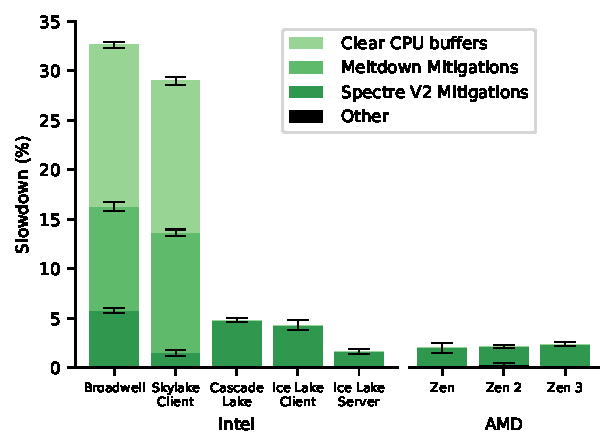
\includegraphics[width=\columnwidth]{plots/lebench.pdf}
    \caption{The overhead of mitigations on the LEBench benchmark suite which stresses the operating system interface. Error bars show 95\% confidence intervals.}
    \label{fig:lebench}
\end{figure}


LEBench~\cite{ren:lebench} is a collection of microbenchmarks for measuring specific operating system operations.\footnote{To align with experiments from elsewhere in this thesis, we use the version of the LEBench benchmarks distributed with \sys~\cite{behrens:ward} .}
In this experiment, we track the geometric mean of benchmarks from the suite.
As seen in \autoref{fig:lebench} the overhead has decreased sharply for newer processors:
CPUs that incorporate hardware mitigations (for Intel) or from a vendor whose CPUs were not vulnerable to all attacks in the first place (AMD) exhibit substantially smaller overheads.

Also notable is that only a small number of mitigations are responsible for nearly all of the overheads.
Collectively, all unlisted mitigations caused a fraction of a percent slowdown on Zen 2, but on the other processors had no statistically-significant impact at all.

\subsection{Octane 2}
\label{sec:benchmarks:octane-2}

\begin{figure}[h]
    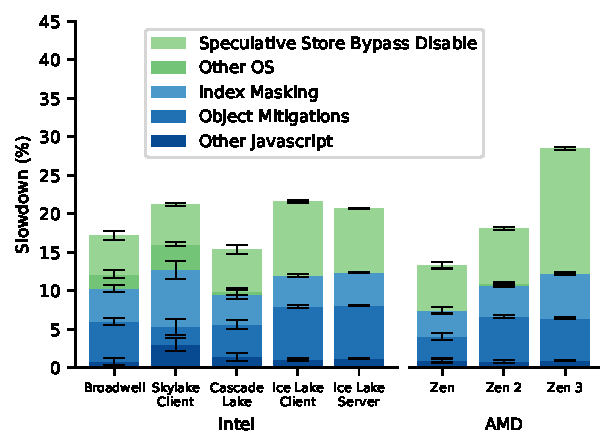
\includegraphics[width=\columnwidth]{plots/octane2.pdf}
    \caption{Slowdown on the Octane 2 browser benchmark caused by JavaScript and operating system level mitigations. Error bars show 95\% confidence intervals.}
    \label{fig:octane2}
\end{figure}

Octane 2 is a benchmark for JavaScript performance, which we run from within Firefox.
\autoref{fig:octane2} plots the percent decrease in scores caused by enabling each mitigation in turn.
JavaScript mitigations (Index masking, object mitigations, and ``other JavaScript'') are shown in blue, while operating system controlled mitigations including Speculative Store Bypass Disable (SSBD) and ``other OS'' are shown above them in green.

All JavaScript mitigations are implemented by the JIT engine inserting extra instructions into the generated instruction stream, and are used to prevent different variations of the Spectre V1 attack.
For instance, index masking ensures that speculative accesses to an array do not index past the end of an array.
It does so by placing a conditional move instruction before every array access which checks whether the access is in bounds and overwrites the index with zero otherwise.
This check overall takes very little time but it prevents the CPU from starting to pull the array contents into cache until the array length is known.
Across many millions of array accesses in the Octane 2 benchmark, this ends up causing a non-trivial cost.

Speculative Store Bypass Disable is an OS level mitigation that is disabled by default for most processes, but on the kernel versions we're using is enabled for Firefox because it uses seccomp.
Starting with Linux 5.16 released in January 2022, the kernel by default no-longer enables the mitigation for seccomp processes~\cite{phoronix:ssbd-defaults}.
Applications can still enable the mitigation manually, but Firefox releases so far don't override the kernel setting.

This may stop being relevant.
Intel has reserved a bit in in the \texttt{ARCH\_CAPABILITIES} model-specific register to indicate that a given processor isn't vulnerable to Speculative Store Bypass and therefore that the associated mitigation is neither needed nor implemented.
However, we do not know of any CPUs for either vendor that set that bit, not even models that came out years after the attack was discovered.

\subsection{Virtual Machine Workloads}
\label{sec:benchmarks:vm}

We measure two different virtual machine workloads relevant to how VMs are used in production.
The performance of running LEBench inside of a virtual machine with and without host mitigations enabled mirrors running a customer application on a cloud provider.
Execution primarily (but not exclusively) stays within the VM so we would expect host mitigations to have limited impact on the performance observed by the guest.
This matches our observations: measured overhead was $\pm 3$\% on all systems, signalling that the mitigations applied by a hypervisor do not have significant impact.
Some runs suggested a slowdown in the range of 1-3\%, but our methodology resulted in too much variability between runs to be confident whether or not that was caused by noise. 
In any case, we were unable to attribute the slowdown to specific mitigations because the slowdowns are so small.

Secondly, we measure the overhead of virtual machine exits by running the \textit{smallfile} and \textit{largefile} microbenchmarks from LFS~\cite{rosenblum:lfs} against an emulated disk.
The median overhead was under $2$\%, but once again, we observed high variability between runs.
This workload performs many security boundary crossings because every access to the emulated disk requires running code within the hypervisor.
However, in contrast to LEBench that reached millions of system calls per second, the higher cost of VM exits meant that this experiment only reached several tens of thousands of VM exits per second.
We believe that this explains the lack of a clear slowdown; the comparatively small number of protection domain crossings means that even though the time spent on mitigations during a single VM exit is likely higher than for a system call, in relative terms it is not enough to meaningfully impact the end-to-end performance.

\subsection{PARSEC}
\label{sec:benchmarks:parsec}
As a final experiment we measure the overhead of running the \textit{swaptions}, \textit{facesim}, and \textit{bodytrack} benchmarks from the PARSEC suite.
These were chosen to get good coverage of compute-intensive benchmarks with different working set sizes.
None involve significant numbers of calls into the operating system nor user-level sandboxing, as explored by the previous experiments, which makes them ideal to measure the impact solely of ``always on'' mitigations that the OS applies to running processes.

We were unable to observe any meaningful difference between running with and without the default set of mitigations: total runtime was usually within $\pm0.5$\% for the two configurations, and never differed by more than $2$\%.
This serves as a reminder that slowdowns from transient execution attack mitigations aren't relevant to all workloads.

The one exception is that we observed significant overheads by force-enabling mitigations for Speculative Store Bypass.
\autoref{sec:ssb} explores this in more detail.

\subsection{Summary}
Each of these benchmarks plots a different trajectory of mitigation costs.
Workloads that stress the operating system interface have received the most attention, and overheads on LEBench have gone from over 30\% on older Intel CPUs to under 3\% on the latest models, thanks to fixes for several of the attacks.
By contrast, none of the attacks impacting JavaScript performance have been addressed in hardware and overhead on Octane 2 has remained in the range of 15\% to 25\%.
Our compute-intensive benchmark has negligible overhead regardless of the processor, and we did not observe significant overheads on either of the two VM workloads measured.
These trends are consistent with prior work from Phoronix~\cite{phoronix:three-years}, which found big improvements on OS workloads (perf-bench, ctx\_clock, etc.), moderate but consistent overheads for web browsers (Selenium), and minimal overheads for the more compute-intensive workloads.

There has been a significant effort from computer architecture researchers towards addressing Spectre V1~\cite{barber:specshield, weisse:nda, ainsworth:muontrap,yu:stt,yu:sdo}, but interestingly software mitigations for the attack had no measurable impact on LEBench performance.
By contrast, they account for around half the overhead on the browser workload.

It is also worth pointing out that all three attacks with significant overhead on new processor are actually quite ``old''.
Spectre V1 and Spectre V2 were the first transient execution attacks discovered (along with Meltdown, which was discovered at the same time), while Speculative Store Bypass followed only a matter of months later.
Over the subsequent three years of transient execution attack discoveries, they've all either been quickly resolved in hardware or had a negligible cost to mitigate in software.
This paints an optimistic outlook for the future (assuming this remains true).
